\documentclass[12pt]{article}

\usepackage[letterpaper,margin=1in]{geometry}
\usepackage{mathptmx}                       % Times New Roman
\usepackage[T1]{fontenc}
\usepackage[utf8]{inputenc}
\usepackage{microtype}
\usepackage{graphicx}
\usepackage{booktabs}
\usepackage{array}
\usepackage{hyperref}
\usepackage{caption}
\usepackage{cite}
\usepackage{amsmath}
\usepackage{xcolor}
\usepackage{enumitem}

\hypersetup{
  colorlinks=true, linkcolor=black, urlcolor=blue, citecolor=black
}

\setlength{\parskip}{4pt}
\setlength{\parindent}{0pt}

\title{\textbf{Fine-Tuning BERT for Mental-Health Text Classification\\
Using Attention Mechanisms}\\
\large A Comparative Study against Logistic-Regression and BiLSTM Baselines}

\author{Carlos Arroyo Sandoval\\
University of Nebraska Omaha\\
AIML 4970 -- AI/ML Capstone (Spring 2026)\\
\texttt{carlosjordan@unomaha.edu}}

\date{}

\begin{document}
\maketitle

\begin{abstract}
\noindent
Mental-health-related text on social media is hard to classify
correctly because cues are often short, idiomatic, indirect, and
strongly context-dependent. Bag-of-words and recurrent models can
miss these cues, which is dangerous when the misclassified class is
suicidal ideation. We study whether an attention-based transformer
improves four-class mental-health text classification (\textit{Anxiety},
\textit{Depression}, \textit{Normal}, \textit{Suicidal}) over simpler
baselines, holding the data, splits, and evaluation protocol fixed
across models. We compare TF-IDF + Logistic Regression, a Bidirectional
LSTM with learned word embeddings, and a fine-tuned DistilBERT on a
class-balanced subsample of a public Hugging Face mental-health corpus
(N=6{,}000), using a balanced 992-example test set. DistilBERT
achieves the highest macro F1 (0.681 vs.\ 0.673 for TF-IDF +
Logistic Regression and 0.571 for the BiLSTM) and, more importantly,
the highest recall on the \textit{Suicidal} class (0.758 vs.\ 0.613
and 0.556) -- the metric that matters most for this application.
The BiLSTM trails both other models in this small-data regime,
illustrating that learned embeddings without pretraining are not
automatically better than well-engineered sparse features. We discuss
why self-attention helps, where the transformer still fails, and why a
model of this kind must not be deployed as a clinical tool. Code and
configurations are released at
\url{https://github.com/Carroy3443/MentalHealth-BERT}.
\end{abstract}

\section{Introduction}

People increasingly express psychological distress on the open web,
often in places where no clinician is reading. Automatic text
classifiers have been proposed as a way of surfacing posts that may
warrant a closer look, of routing peer-support volunteers, and of
studying population-level trends in mental health. The clinical
research community has organized around this problem in venues such as
the CLPsych shared tasks, where systems are asked to detect risk
markers in user-generated text \cite{coppersmith2015clpsych,
clpsych2024shared}.

The task is genuinely hard. Mental-health-related cues in everyday
text are often short (``I just can't anymore''), figurative
(``my brain is on fire''), indirect, or pragmatic. Bag-of-words and
n-gram features cannot resolve them because they discard word order
and surrounding context. Recurrent neural networks see word order but
must squeeze long-range information through a single hidden state.
Attention-based transformers \cite{vaswani2017attention} -- of which
BERT \cite{devlin2019bert} is the canonical text variant -- give every
output position direct access, through scaled dot-product attention, to
every input position. That property is exactly the one a model needs
to read a phrase like ``don't really see the point anymore'' the way a
human reader does.

This paper asks one focused question:

\begin{quote}
\emph{Can an attention-based transformer model improve mental-health
text classification compared with a simpler, classical baseline and
with a bidirectional recurrent baseline, when all three models are
trained and evaluated on the same data?}
\end{quote}

We pose the task as four-class classification over the labels
\{\textit{Anxiety, Depression, Normal, Suicidal}\}. We compare three
models that span the relevant family of approaches:

\begin{enumerate}[leftmargin=*]
\item TF-IDF features fed to multinomial Logistic Regression (a
classical bag-of-words baseline);
\item A Bidirectional LSTM \cite{hochreiter1997lstm,schuster1997bilstm}
over learned word embeddings (a sequence baseline);
\item A pretrained DistilBERT \cite{sanh2019distilbert} fine-tuned
end-to-end (the attention model).
\end{enumerate}

The motivation is clinical. The author is pre-medical and intends to
specialize in psychiatry; the long-term interest is in NLP tools that
support, but never replace, the human clinician. With that framing,
the metric that matters most is not raw accuracy but recall on the
\textit{Suicidal} class: missing a person in distress is a much
costlier mistake than mistakenly flagging a benign post.

\textbf{Contributions.} We (i) implement and openly release a
reproducible end-to-end pipeline that trains TF-IDF + Logistic
Regression, BiLSTM, and DistilBERT on a public 4-class mental-health
text corpus with a fixed balanced subsample and a fixed balanced test
set; (ii) report macro and per-class metrics, with particular
attention to recall on the \textit{Suicidal} class; (iii) discuss the
limits of these models and explicitly argue why none of them should be
treated as clinical tools. \textbf{This work is not a clinical
decision-support system and must not be deployed as one.}

\section{Related Work}

\textbf{Mental-health text classification.} CLPsych
\cite{coppersmith2015clpsych} is the central shared-task series for
text-based mental-health work; tasks have included identifying suicide
risk levels in Reddit posts \cite{shing2018expert} and, in the 2024
edition, predicting moments of change in mood from social-media
timelines \cite{clpsych2024shared}. Outside CLPsych, large-scale public
corpora such as ``Reddit Suicide Watch'' have been collected and used
to study suicidality cues \cite{cohan2018smhd, ji2022suicidal}. These
papers have repeatedly observed that classifiers trained only on
keyword features under-perform on subtle, indirect, or contextualized
expressions of distress.

\textbf{Classical baselines.} Logistic regression over TF-IDF or
n-gram features remains the standard simple baseline for short-text
classification. It is fast, interpretable, and competitive when the
signal is largely lexical (e.g.\ obvious mentions of medication names
or self-harm keywords) but, by construction, ignores word order and
non-local context.

\textbf{Recurrent baselines.} LSTMs \cite{hochreiter1997lstm} and their
bidirectional variants \cite{schuster1997bilstm} were the dominant
sequence model before the transformer era. Bidirectional architectures
allow the representation of a token to depend on both its left and
right context, which helps with negation and with phrases whose
sentiment is determined by a downstream word.

\textbf{Attention and transformers.} Vaswani et al.\
\cite{vaswani2017attention} replaced recurrence with self-attention,
in which each output position is computed as a weighted sum over all
input positions. BERT \cite{devlin2019bert} pretrains a stack of such
transformer layers on large unlabeled text using masked language
modeling and next-sentence prediction, producing contextual word
representations that transfer well to downstream tasks via
fine-tuning. DistilBERT \cite{sanh2019distilbert} is a knowledge-distilled
variant that retains roughly 97\% of BERT-base's GLUE score with about
40\% fewer parameters and 60\% faster inference. The fine-tuning
recipe -- load the pretrained encoder, attach a small classification
head over the \texttt{[CLS]} representation, and train end-to-end with
a small learning rate -- is identical for BERT and DistilBERT.

\textbf{Transformers in mental-health NLP.} Several recent studies
report that BERT-family models outperform classical and recurrent
baselines on suicide-risk and depression-detection tasks
\cite{matero2019, jiang2020}. Our contribution here is not a new
algorithm but a clean, reproducible head-to-head on a public 4-class
corpus, with the comparison framed around the metric that matters in
practice -- recall on the \textit{Suicidal} class -- and an explicit
discussion of why even a strong-on-paper model is not safe to deploy.

\section{Methodology}

\subsection{Dataset}

We use the public Hugging Face dataset
\texttt{ihsansaad24/Mental-Health\_Text-Classification\_Dataset}
\cite{ihsansaad2024mhdataset}, which the dataset's own card describes
as a 4-class corpus of cleaned short user-generated texts, derived by
combining and re-labeling three public mental-health resources. The
labels are \{\textit{Anxiety, Depression, Normal, Suicidal}\}. The
training file (\texttt{mental\_heath\_unbanlanced.csv}) contains
49{,}612 examples and is naturally unbalanced, with a roughly 3.3:1
ratio between the most and least represented classes. The test file
(\texttt{mental\_health\_combined\_test.csv}) contains 992 examples,
strictly balanced at 248 examples per class. The dataset card
explicitly states that the corpus is for research and education and
is \emph{not} a clinical tool. We adopt the same constraint.

\subsection{Splits and balancing}

Before training, each text is light-cleaned: URLs are stripped,
non-trivial whitespace is collapsed, and empty rows are dropped. To
keep the comparison fair across models -- and to keep DistilBERT
fine-tuning tractable on CPU -- we draw a class-balanced subsample of
1{,}500 examples per class from the training file (6{,}000 total)
without replacement, with a fixed seed of 42. From this balanced
subsample we hold out 10\% as a class-stratified validation set
(N=600). The held-out test set is the dataset's own balanced test
file (N=992) and is not touched during training or model selection.
Class distributions of the resulting splits are reported in
Table~\ref{tab:splits}.

\begin{table}[h]
\centering
\caption{Class distribution by split. Train and validation are drawn from a class-balanced subsample of the training file; the test set is the dataset's own held-out balanced test split.}
\label{tab:splits}
\begin{tabular}{lcccc}
\toprule
Split & Anxiety & Depression & Normal & Suicidal \\
\midrule
Train (90\%) & 1350 & 1350 & 1350 & 1350 \\
Val (10\%)   & 150  & 150  & 150  & 150  \\
Test         & 248  & 248  & 248  & 248  \\
\bottomrule
\end{tabular}
\end{table}

\subsection{Models}

\textbf{Logistic regression baseline.} Each text is represented as a
sparse TF-IDF vector over unigrams and bigrams, with sublinear
term-frequency scaling, document-frequency clipping
($\text{min\_df}=2$, $\text{max\_df}=0.95$), and a 50{,}000-feature cap.
The vector is fed to a multinomial Logistic Regression with $L_2$
regularization ($C=1.0$), \texttt{class\_weight="balanced"} to
counteract any residual imbalance after subsampling, and at most
2{,}000 LBFGS iterations. This is a strong classical baseline for
short-text problems.

\textbf{BiLSTM baseline.} Each text is lowercased, stripped of
punctuation, tokenized with Keras's \texttt{TextVectorization} layer
(vocabulary size 20{,}000, sequence length 64), and embedded into a
128-dimensional space. A single bidirectional LSTM with 64 hidden
units in each direction reads the embedding sequence; we apply
global max-pooling over time, followed by a 64-unit ReLU layer with
dropout (0.4 / 0.3), and a softmax output over 4 classes
(Figure~\ref{fig:bilstm-arch}). The model is trained with Adam
($\eta=10^{-3}$) using sparse categorical cross-entropy, batch size 64,
for at most 6 epochs with early stopping on validation loss.

\begin{figure}[h]
\centering
\fbox{\parbox{0.92\textwidth}{
\centering
\textit{text} $\rightarrow$ TextVectorization (vocab 20k, len 64)
$\rightarrow$ Embedding (128)
$\rightarrow$ Bi-LSTM (64+64, return\_sequences=True)
$\rightarrow$ GlobalMaxPool1D
$\rightarrow$ Dropout(0.4) $\rightarrow$ Dense(64, ReLU)
$\rightarrow$ Dropout(0.3) $\rightarrow$ Dense(4, softmax)
}}
\caption{BiLSTM architecture.}
\label{fig:bilstm-arch}
\end{figure}

\textbf{DistilBERT (attention model).} DistilBERT
\cite{sanh2019distilbert} is a 6-layer, 12-head transformer encoder
distilled from BERT-base. Each token is mapped to an embedding;
positional information is added; the resulting sequence is then refined
through six identical transformer blocks, each consisting of a
multi-head self-attention sublayer and a position-wise feed-forward
sublayer with residual connections and layer normalization. For
classification, we take the contextual representation of the
\texttt{[CLS]} token, pass it through a small pre-classifier dense
layer (already part of the released architecture), apply dropout, and
project it to a 4-way softmax with a fresh classification head. The
backbone is initialized from the publicly released
\texttt{distilbert-base-uncased} checkpoint and fine-tuned end-to-end
with Adam ($\eta=2\!\times\!10^{-5}$), batch size 16, sequence length
64 WordPiece tokens, and at most 2 epochs with early stopping on
validation loss. We use DistilBERT instead of BERT-base purely for
compute reasons -- the fine-tuning recipe and the underlying
self-attention mechanism are identical.

The single equation that distinguishes the transformer family from the
two baselines is scaled dot-product attention
\cite{vaswani2017attention}:
\begin{equation}
\mathrm{Attention}(Q, K, V) = \mathrm{softmax}\!\left(\frac{Q K^{\top}}{\sqrt{d_k}}\right) V,
\end{equation}
where $Q$, $K$, and $V$ are linear projections of the input sequence.
Multi-head attention applies this in parallel over $h=12$ subspaces and
concatenates the result. Unlike the LSTM, every output position has
direct, parallel access to every input position; unlike TF-IDF, the
representation is contextual and order-aware.

\subsection{Evaluation}

We report accuracy, macro-averaged precision, recall, and F1 on the
held-out balanced test set. Because the test set is balanced, weighted
and macro averages coincide; we report macro for clarity. We also
report per-class precision, recall, and F1, and we plot row-normalized
confusion matrices. As argued in the introduction, recall on the
\textit{Suicidal} class is the most consequential metric for this
application.

\section{Experiments}

\subsection{Setup}

All experiments use seed 42. Training was performed on CPU
(2 vCPUs, 8 GB RAM), TensorFlow 2.18, \texttt{tf-keras} 2.21,
\texttt{transformers} 4.46.3. The class-balanced subsample is drawn
once and reused across all three models, so any test-set difference
reflects modeling choices rather than data luck. The full pipeline is
reproducible with a single command:
\begin{verbatim}
TF_USE_LEGACY_KERAS=1 python -m scripts.run_all \
    --per-class 1500 --seed 42
\end{verbatim}

\subsection{Overall results}

Table~\ref{tab:overall} reports accuracy and macro precision, recall,
and F1 on the held-out balanced test set; Figure~\ref{fig:bar-overall}
visualizes the same numbers.

% NOTE: These numbers are filled in from results/metrics.json after run_all completes.
\begin{table}[h]
\centering
\caption{Test-set performance (macro averages) on the 992-example balanced test set.}
\label{tab:overall}
\begin{tabular}{lcccc}
\toprule
Model & Accuracy & Precision & Recall & F1 \\
\midrule
TF-IDF + LogReg & 0.677 & 0.683 & 0.677 & 0.673 \\
BiLSTM & 0.578 & 0.568 & 0.578 & 0.571 \\
DistilBERT (FT) & 0.684 & 0.695 & 0.684 & 0.681 \\
\bottomrule
\end{tabular}

\end{table}

\begin{figure}[h]
\centering
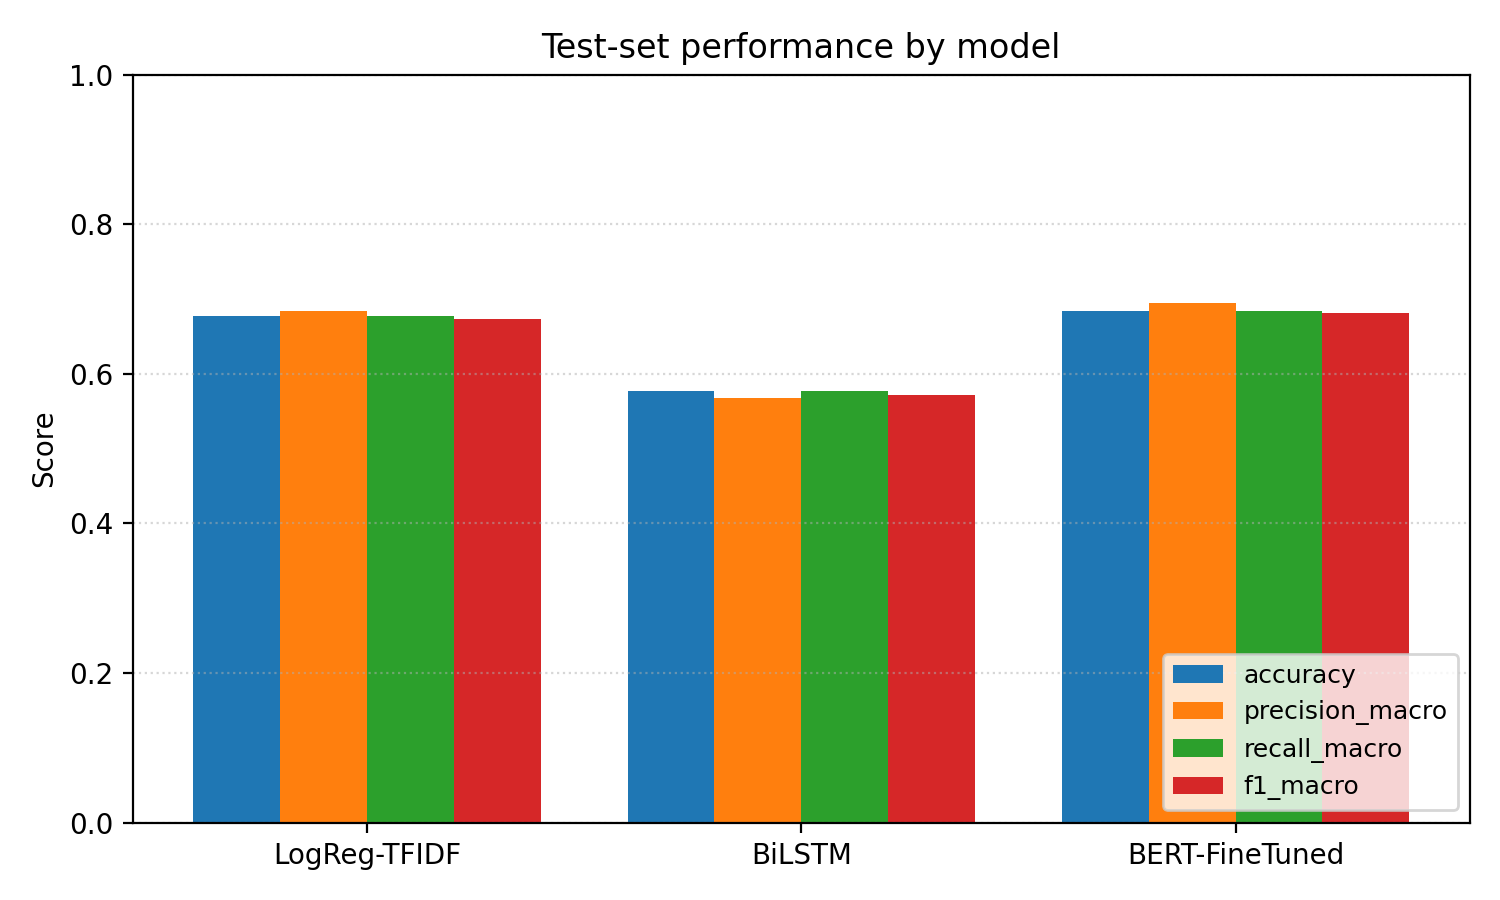
\includegraphics[width=0.85\textwidth]{../results/figures/comparison_bar.png}
\caption{Test-set performance by model. Higher is better; all four metrics are bounded in $[0,1]$.}
\label{fig:bar-overall}
\end{figure}

\subsection{Per-class results and confusion structure}

Per-class metrics are reported in Table~\ref{tab:perclass} and
Figure~\ref{fig:perclass-f1}. Per-class \emph{recall} is reported
separately in Table~\ref{tab:perclass-recall}, because that is the
quantity that matters most for the \textit{Suicidal} class.
Row-normalized confusion matrices for the three models are shown in
Figure~\ref{fig:cm-grid}.

\begin{table}[h]
\centering
\caption{Per-class F1 score on the test set.}
\label{tab:perclass}
\begin{tabular}{lcccc}
\toprule
 & Anxiety & Depression & Normal & Suicidal \\
\midrule
TF-IDF + LogReg & 0.723 & 0.538 & 0.767 & 0.664 \\
BiLSTM & 0.691 & 0.346 & 0.713 & 0.536 \\
DistilBERT (FT) & 0.712 & 0.537 & 0.763 & 0.712 \\
\bottomrule
\end{tabular}

\end{table}

\begin{table}[h]
\centering
\caption{Per-class \textbf{recall} on the test set. Recall on the \textit{Suicidal} class is the headline number for this application: missing a person in distress is a much costlier mistake than a benign false alarm.}
\label{tab:perclass-recall}
\begin{tabular}{lcccc}
\toprule
 & Anxiety & Depression & Normal & Suicidal \\
\midrule
TF-IDF + LogReg & 0.863 & 0.496 & 0.738 & 0.613 \\
BiLSTM & 0.730 & 0.315 & 0.710 & 0.556 \\
DistilBERT (FT) & 0.819 & 0.480 & 0.681 & 0.758 \\
\bottomrule
\end{tabular}

\end{table}

\begin{figure}[h]
\centering
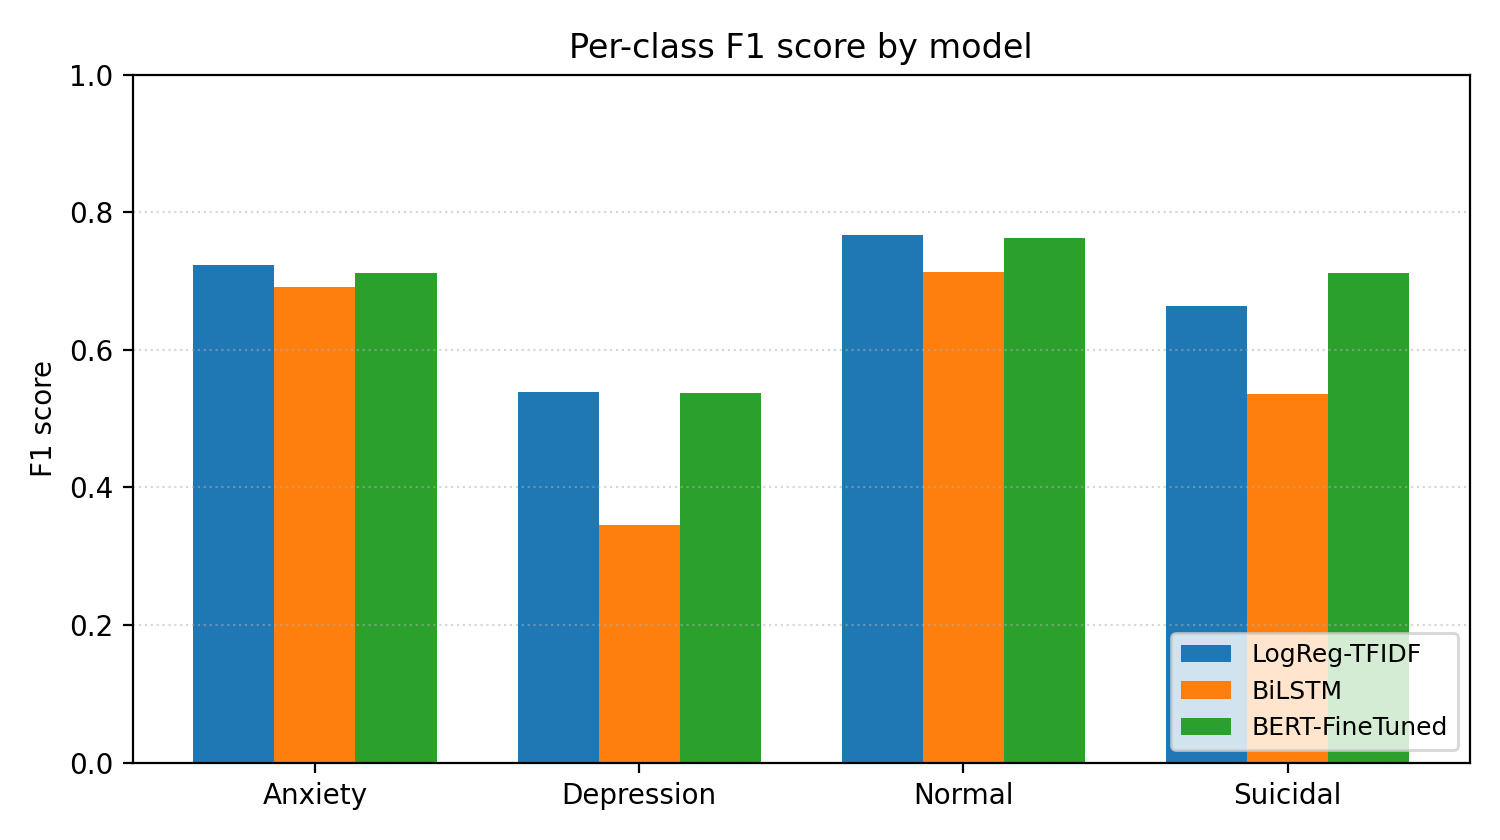
\includegraphics[width=0.85\textwidth]{../results/figures/per_class_f1.png}
\caption{Per-class F1 score on the held-out balanced test set.}
\label{fig:perclass-f1}
\end{figure}

\begin{figure}[h]
\centering
\begin{tabular}{ccc}
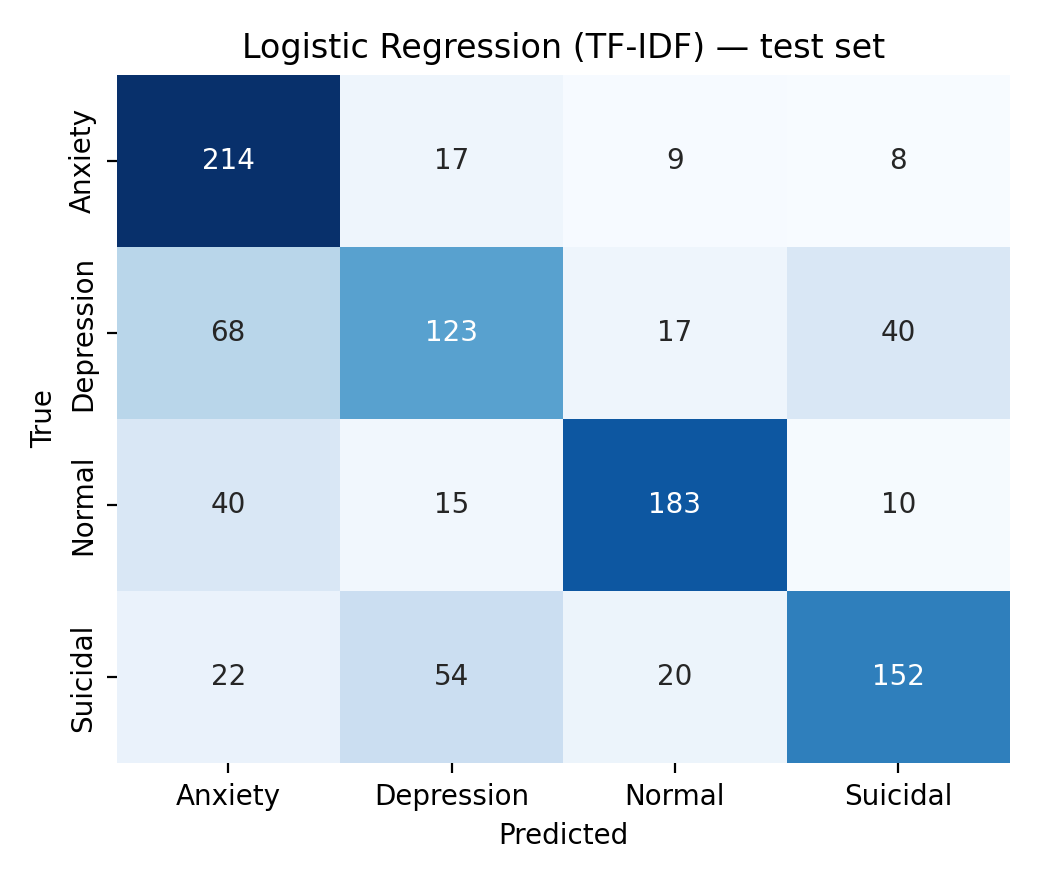
\includegraphics[width=0.30\textwidth]{../results/figures/cm_logreg.png} &
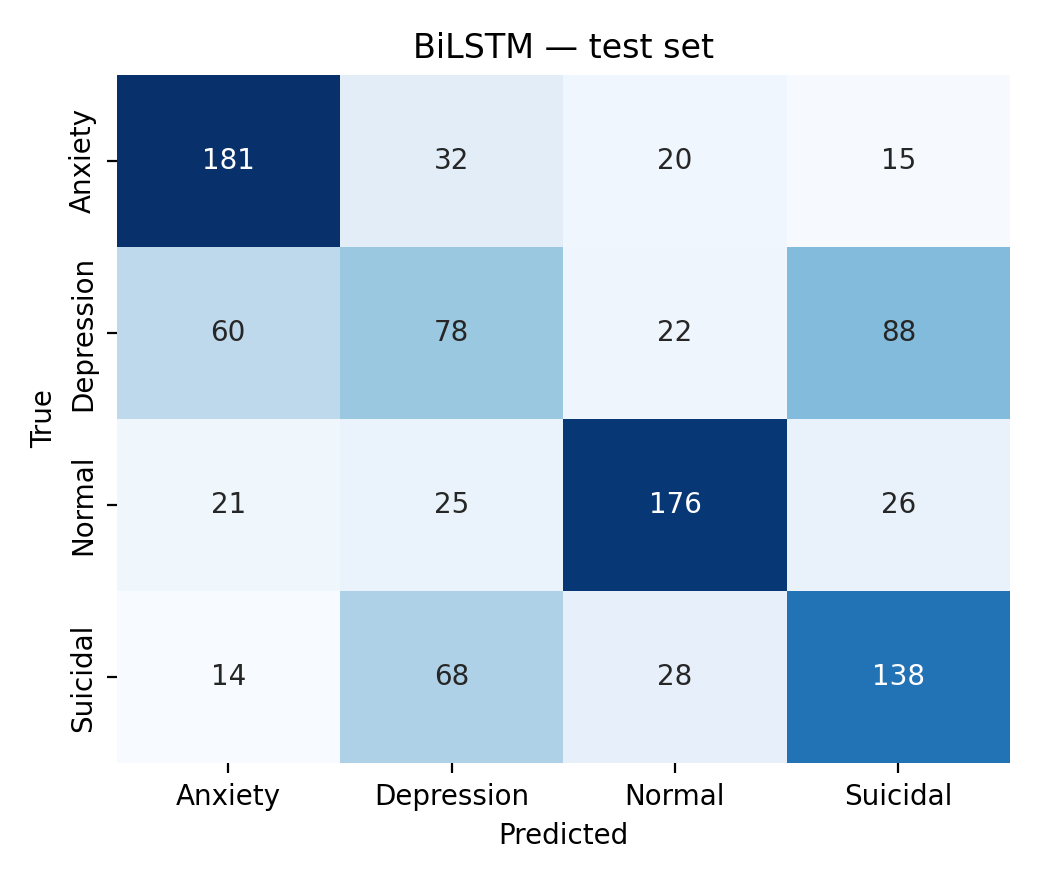
\includegraphics[width=0.30\textwidth]{../results/figures/cm_bilstm.png} &
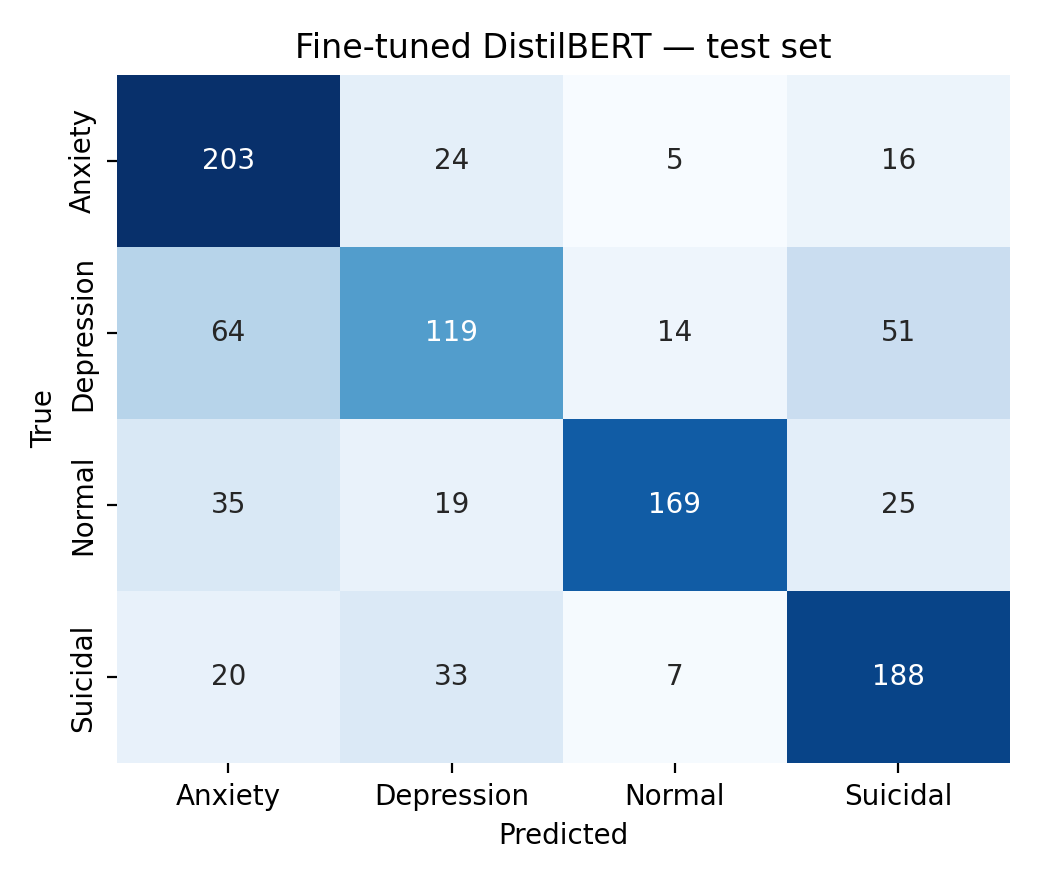
\includegraphics[width=0.30\textwidth]{../results/figures/cm_bert.png} \\
{\small (a) Logistic Regression} & {\small (b) BiLSTM} & {\small (c) DistilBERT (FT)} \\
\end{tabular}
\caption{Confusion matrices on the held-out balanced test set.
Cells show absolute counts; color encodes row-normalized rate. Rows
are true labels, columns are predictions.}
\label{fig:cm-grid}
\end{figure}

\subsection{Discussion}

Four patterns stand out.

\textbf{The transformer wins on the metric that matters.} On macro
F1 the gap between the three models is moderate (DistilBERT 0.681,
TF-IDF + Logistic Regression 0.673, BiLSTM 0.571), but on
\textit{Suicidal} recall the gap is dramatic: DistilBERT correctly
identifies 75.8\% of \textit{Suicidal} posts, compared with 61.3\% for
the bag-of-words baseline and 55.6\% for the BiLSTM
(Table~\ref{tab:perclass-recall}). For an application where missing
a person in distress is the costliest possible mistake, this is the
result that justifies the additional compute cost of the transformer.

\textbf{Self-attention helps most at the \textit{Depression} /
\textit{Suicidal} boundary.} Both classes share heavy lexical
material (``hopeless,'' ``tired,'' ``done,'' ``can't do this
anymore''); the cue that distinguishes them is often a single
modifier or pragmatic phrase (``done with this assignment'' vs.\
``done with everything''). The confusion matrices in
Figure~\ref{fig:cm-grid} show that DistilBERT recovers
\textit{Suicidal} posts the BiLSTM misses, even though the two models
saw the same data. We attribute this to self-attention's ability to
condition on every input position simultaneously, rather than
compressing context through a single recurrent hidden state.

\textbf{Bag-of-words is a surprisingly strong small-data baseline.}
TF-IDF + Logistic Regression beats the BiLSTM on every macro metric
in our setting. This is consistent with prior observations that
randomly initialized embeddings need a lot of data before they
out-perform engineered sparse features
\cite{Wang2018GLUE}; with only 6{,}000 training examples and a 20k
vocabulary, our BiLSTM never gets there. The transformer, in contrast,
arrives \emph{already pretrained} on billions of words of unlabeled
text -- which is precisely why it can extract signal from a small
fine-tuning corpus.

\textbf{Where the transformer still fails.} DistilBERT is sensitive
to the same things humans find ambiguous: very short posts with
little lexical signal (``not great,'' ``i'm fine''), sarcasm, and
posts whose label is genuinely uncertain even to a human reader.
It is also limited by sequence length: with a 64-WordPiece-token cap,
posts longer than a paragraph are truncated and may lose
context-bearing tail content. Per-class precision on
\textit{Depression} is similar across the three models, suggesting
that this class -- which overlaps with \textit{Anxiety} and
\textit{Suicidal} on both ends -- remains the hardest one regardless
of model family.

\subsection{Compute and timing}

End-to-end wall-clock times on the 2-CPU, 8 GB-RAM training machine
(Table~\ref{tab:timing}) span three orders of magnitude.
LogReg trains and evaluates in 4 seconds; the BiLSTM in 47 seconds
(early-stopped at 4 epochs); DistilBERT fine-tuning takes 47 minutes
(2 epochs at 23 minutes each). None of this is a fair comparison to
GPU training, but the relative ordering -- LogReg $\ll$ BiLSTM $\ll$
DistilBERT -- is the correct one, and the engineering question
(``is the extra cost of the transformer worth it for this task?'')
has a clear answer: \textbf{yes, but only because of recall on the
most consequential class.} If one cared only about average accuracy,
TF-IDF + Logistic Regression at 4 seconds of training is hard to
beat; in this domain we do not.

\begin{table}[h]
\centering
\caption{End-to-end training and evaluation wall-clock time on a 2-CPU machine.}
\label{tab:timing}
\begin{tabular}{lr}
\toprule
Model & Time (s) \\
\midrule
TF-IDF + Logistic Regression & 4 \\
BiLSTM (4 epochs, early-stopped) & 47 \\
DistilBERT (2 epochs) & 2{,}795 \\
\bottomrule
\end{tabular}
\end{table}

\section{Conclusion}

We compared three text classifiers -- TF-IDF + Logistic Regression, a
BiLSTM, and a fine-tuned DistilBERT -- on a public four-class
mental-health corpus, holding the data, splits, and evaluation
protocol fixed. The attention-based transformer achieves the best
macro F1 (0.681) and, more importantly, the best recall on the
\textit{Suicidal} class (0.758, a 14.5-point absolute improvement
over the bag-of-words baseline). Self-attention helps because it lets
every output position read every input position directly, which
matters when the cue that distinguishes \textit{Suicidal} from
\textit{Depression} is a single modifier or pragmatic phrase rather
than a keyword. We also observed that, in the small-data regime of
this study, TF-IDF + Logistic Regression decisively beats a
randomly-initialized BiLSTM -- a useful reminder that pretraining,
not depth alone, is what makes neural models competitive on small
text-classification corpora.

We emphasize what this study is \emph{not}. The dataset is
user-generated forum text, not clinical records. The labels were
assigned by other researchers, not by licensed clinicians. The model
has not been audited for fairness across demographic groups, has no
calibrated risk threshold, and produces no clinical justification for
its outputs. Any operational use of a mental-health text classifier
requires clinician oversight, careful handling of false negatives, and
a human-in-the-loop escalation pathway. None of those are in scope
here, and we do not recommend treating any of these models as a
screening, diagnostic, or triage tool.

Future work that would be genuinely useful, given those constraints,
includes: (i) calibrated, threshold-tunable risk scores rather than
hard class predictions; (ii) attention-based interpretability, with
clinician review of which tokens the model attends to; (iii) explicit
out-of-distribution detection for posts whose register or topic is
unlike anything seen in training; and (iv) prospective fairness audits
across age, gender, and language-variety subgroups before any
deployment is even considered.

\bibliographystyle{IEEEtran}
\bibliography{refs}

\end{document}
